\documentclass[10pt,a4paper]{article}

\usepackage[margin=0.62in]{geometry}
\usepackage{graphicx}
\usepackage{booktabs}
\usepackage{array}
\usepackage{xcolor}
\usepackage{titlesec}
\usepackage{enumitem}
\usepackage{multicol}
\usepackage{tikz}
\usepackage{float}
\usepackage{hyperref}
\usepackage{caption}
\usepackage{fancyhdr}

\usetikzlibrary{arrows.meta, positioning, shapes.geometric}

\definecolor{primary}{HTML}{0B3D2E}
\definecolor{accent}{HTML}{C75B12}
\definecolor{softgray}{HTML}{F4F6F5}

\hypersetup{
    colorlinks=true,
    linkcolor=primary,
    urlcolor=accent
}

\pagestyle{fancy}
\fancyhf{}
\lhead{\textcolor{primary}{Forest Firefighting Robotics Mission}}
\rhead{\textcolor{primary}{Webots + Drone/Ground Team}}
\cfoot{\thepage}

\titleformat{\section}
  {\large\bfseries\color{primary}}
  {\thesection}{0.5em}{}

\titleformat{\subsection}
  {\normalsize\bfseries\color{accent}}
  {\thesubsection}{0.5em}{}

\setlist[itemize]{leftmargin=1.2em, itemsep=1pt, topsep=2pt}
\setlength{\parindent}{0pt}
\setlength{\parskip}{4pt}


\IfFileExists{images/muk-logo.png}{
\includegraphics[width=1\textwidth]{images/muk-logo.png}\\[1.0em]}{}


\begin{document}
\begin{center}
    {\Large \textbf{\textcolor{primary}{Autonomous Forest Firefighting Mission using Webots Robots}}}\\[6pt]
    {\large \textsc{Robotics Practical Simulation Test}}\\[16pt]

    \textbf{Student Details (Day Class)}\\[6pt]
    \begin{tabular}{@{} l l l @{}}
    \toprule
    \textbf{Name} & \textbf{Student Number} & \textbf{Registration Number} \\
    \midrule
    Wangoda Francis & 2400711855 & 24/U/11855/PS \\
    \bottomrule
    \end{tabular}\\[16pt]
    \textbf{Repository URL}\\[6pt]
    \url{https://github.com/WangodaFrancis667/forest-firefighters.git}
\end{center}

\vspace{-0.4em}

\section{Introduction}
This project implements an autonomous forest firefighting mission in the Webots Forest Firefighters simulation environment. The mission objective is to use robots to patrol a forest, detect fire or smoke using onboard cameras, navigate toward the detected fire, and extinguish it by dropping water. The original project baseline is retained in the \texttt{original/} folder for review and comparison. The active solution extends that working baseline from two Mavic drones to four Mavic drone controllers deployed across the four forest quadrants, supported by the Spot-like ground robot. This configuration restores the reliable original detection style while adding the two missing aerial robots needed for full quadrant coverage on the NVIDIA RTX A1000 6 GB GPU.

The implementation was executed in a stable Webots R2021b Docker environment with NVIDIA GPU OpenGL rendering. Before each mission test, a preflight checker verified that all four drones started from separate quadrant base positions:
\begin{itemize}
    \item \textbf{SW Quadrant}: Drone 1 at $(4.0, 4.0, 17.4)$
    \item \textbf{NW Quadrant}: Drone 2 at $(2.0, 26.0, 18.82)$
    \item \textbf{SE Quadrant}: Drone 3 at $(26.0, 3.0, 15.25)$
    \item \textbf{NE Quadrant}: Drone 4 at $(28.0, 26.0, 19.34)$
\end{itemize}
This ensured that all later results measured mission behaviour rather than incorrect spawn placement.

\section{System Architecture}
The system is organised as a closed-loop multi-robot firefighting pipeline. The Webots world provides terrain, fire propagation, smoke, robot bodies, sensors, and the water-drop mechanism. The four Mavic drones provide aerial coverage, camera perception, GPS localisation, and stabilised flight. The fire supervisor starts the wildfire after 40 seconds, giving the drones time to launch while still forcing an early detection and response phase. The Spot-like ground robot remains active as a stable support platform with a keyboard-triggered water burst.

\begin{figure}[H]
\centering
\resizebox{0.96\linewidth}{!}{%
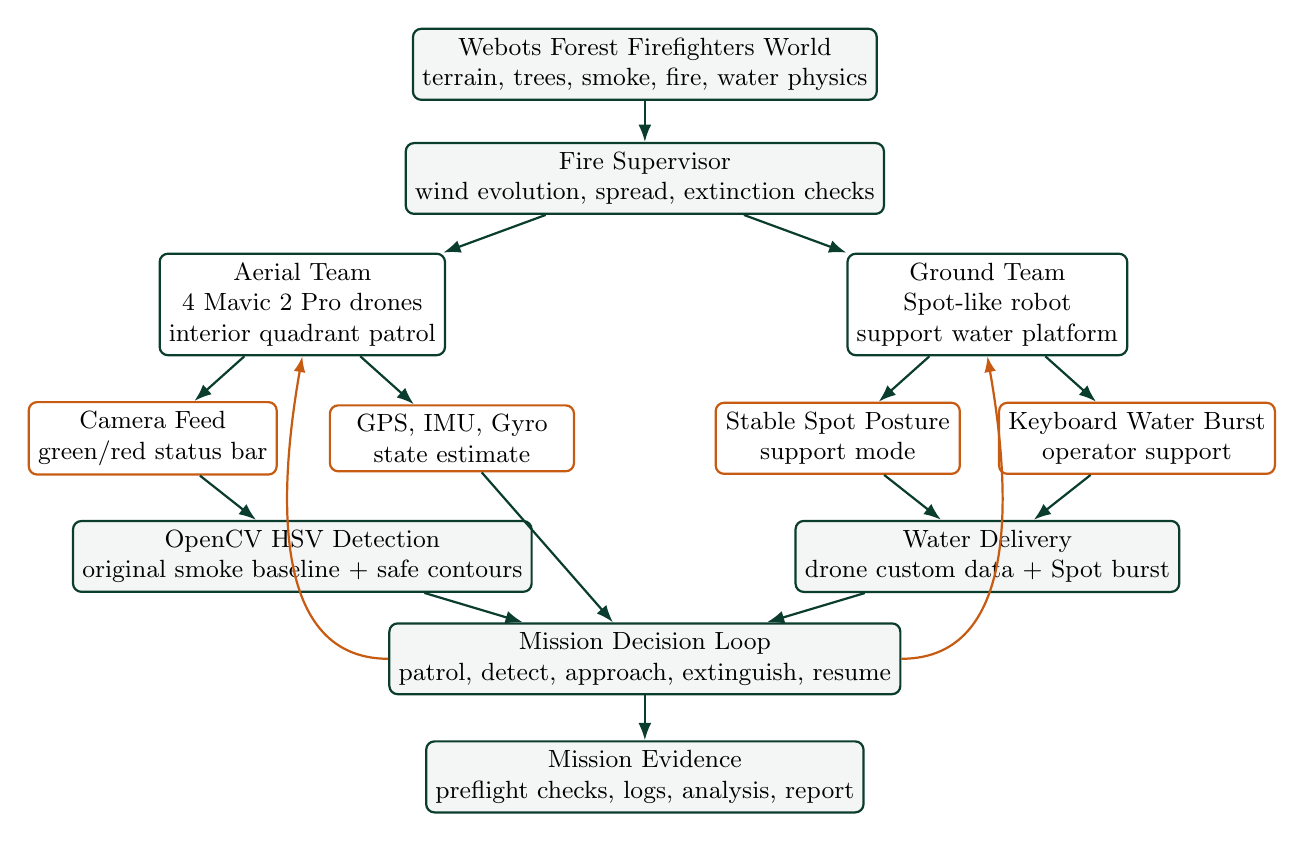
\begin{tikzpicture}[
    system/.style={rectangle, rounded corners=3pt, draw=primary, fill=softgray, thick, align=center, minimum width=3.3cm, minimum height=0.75cm, font=\small},
    team/.style={rectangle, rounded corners=3pt, draw=primary, fill=white, thick, align=center, minimum width=3.5cm, minimum height=0.85cm, font=\small},
    process/.style={rectangle, rounded corners=3pt, draw=accent, fill=white, thick, align=center, minimum width=3.1cm, minimum height=0.7cm, font=\small},
    action/.style={rectangle, rounded corners=3pt, draw=primary, fill=softgray, thick, align=center, minimum width=4.0cm, minimum height=0.8cm, font=\small},
    arrow/.style={-{Latex[length=2.2mm]}, thick, color=primary},
    softarrow/.style={-{Latex[length=2mm]}, thick, color=accent}
]
\node[system] (world) at (0,0) {Webots Forest Firefighters World\\terrain, trees, smoke, fire, water physics};
\node[system] (supervisor) at (0,-1.45) {Fire Supervisor\\wind evolution, spread, extinction checks};

\node[team] (mavic) at (-4.35,-3.05) {Aerial Team\\4 Mavic 2 Pro drones\\interior quadrant patrol};
\node[team] (spot) at (4.35,-3.05) {Ground Team\\Spot-like robot\\support water platform};

\node[process] (vision) at (-6.25,-4.75) {Camera Feed\\green/red status bar};
\node[process] (state) at (-2.45,-4.75) {GPS, IMU, Gyro\\state estimate};
\node[process] (posture) at (2.45,-4.75) {Stable Spot Posture\\support mode};
\node[process] (manual) at (6.25,-4.75) {Keyboard Water Burst\\operator support};

\node[action] (detect) at (-4.35,-6.25) {OpenCV HSV Detection\\original smoke baseline + safe contours};
\node[action] (nav) at (0,-7.55) {Mission Decision Loop\\patrol, detect, approach, extinguish, resume};
\node[action] (drop) at (4.35,-6.25) {Water Delivery\\drone custom data + Spot burst};
\node[action] (logs) at (0,-9.05) {Mission Evidence\\preflight checks, logs, analysis, report};

\draw[arrow] (world) -- (supervisor);
\draw[arrow] (supervisor) -- (mavic);
\draw[arrow] (supervisor) -- (spot);

\draw[arrow] (mavic) -- (vision);
\draw[arrow] (mavic) -- (state);
\draw[arrow] (spot) -- (posture);
\draw[arrow] (spot) -- (manual);

\draw[arrow] (vision) -- (detect);
\draw[arrow] (state) -- (nav);
\draw[arrow] (posture) -- (drop);
\draw[arrow] (manual) -- (drop);
\draw[arrow] (detect) -- (nav);
\draw[arrow] (drop) -- (nav);
\draw[arrow] (nav) -- (logs);
\draw[softarrow] (nav.west) to[out=180,in=260] (mavic.south);
\draw[softarrow] (nav.east) to[out=0,in=280] (spot.south);
\end{tikzpicture}
}
\caption{System architecture for the final four-drone and Spot firefighting team.}
\end{figure}

\vspace{-0.6em}

\newpage
\section{Methodology and Key Algorithms}
\subsection{Locomotion and Stabilisation}
The Mavic drone is controlled using four propeller motors. The controller computes motor velocities from vertical thrust, roll, pitch, yaw, and altitude error. GPS provides position and altitude feedback, while the inertial unit and gyro provide orientation and angular velocity. The final tuning increases yaw and forward pitch authority relative to the original baseline so the drones patrol and approach detected fire more quickly while remaining stable.

\subsection{Waypoint Patrol Navigation}
Each drone receives patrol coordinates through controller arguments in the world file. The controller stores these coordinates as a waypoint list. During flight, the drone compares its GPS position with the current target waypoint. When it reaches the waypoint within the precision threshold, it automatically switches to the next target. This implements continuous patrol of the forest area.

\subsection{Camera-Based Fire and Smoke Detection}
The onboard camera captures a downward-facing image. The image is converted into an OpenCV-compatible format and then transformed into HSV colour space. The detector uses the original working smoke threshold as the baseline, with safe contour handling added so empty masks cannot crash the controller. The manual display overlay intentionally avoids tree boxes and contour clutter: each drone shows a green top status bar during normal patrol and a red \texttt{FIRE} bar when a fire target is active. The output is an image coordinate $(x,y)$ used by the approach controller.

\subsection{Fire Approach and Water Drop}
After a fire is detected, the controller compares the detected image coordinate with the centre of the camera frame. If the fire is not centred, yaw and pitch disturbances guide the drone toward it. When the fire is centred below the drone, the controller triggers a water-drop command using the drone custom data field. The drone then clears the current target and continues the patrol loop, allowing it to respond to additional propagated fires.

\subsection{Spot Ground Robot Support}
The Spot-like robot is retained from the original project baseline as a ground support robot. Its controller keeps it alive for the full mission, holds a stable support posture, and accepts a keyboard-triggered water burst. In the final architecture, Spot is not the main search platform; it provides visible legged-robot integration and a secondary water-delivery path while the Mavic drones perform wide-area patrol and visual detection.

\section{Performance Results}
The final system was validated using eight mission runs with the active four-drone plus Spot configuration. Each run first passed the preflight check for drone count, launch position, controller assignment, patrol routing, camera/display size, fire start delay, and mission duration.

\begin{table}[H]
\centering
\caption{Mission performance across final four-drone validation runs.}
\small
\resizebox{\linewidth}{!}{%
\begin{tabular}{lrrrrrr}
\toprule
Run & Detections & Drops & Targets & Errors & Crashes & Shutdown Artifacts \\
\midrule
demo & 160 & 10 & 29 & 0 & 0 & 1 \\
final\_demo\_test & 120 & 6 & 31 & 0 & 0 & 0 \\
live\_demo\_final & 162 & 7 & 29 & 0 & 0 & 16 \\
live\_demo\_run & 63 & 4 & 34 & 0 & 0 & 0 \\
stability\_repeat\_01 & 114 & 7 & 30 & 0 & 0 & 16 \\
stability\_repeat\_02 & 75 & 4 & 16 & 0 & 0 & 16 \\
stability\_repeat\_03 & 17 & 4 & 17 & 0 & 0 & 16 \\
stability\_test\_01 & 7 & 1 & 37 & 0 & 0 & 0 \\
baseline\_run & 4 & 1 & 31 & 0 & 0 & 0 \\
\bottomrule
\end{tabular}
}
\end{table}

Across the final validation set, the system produced 718 camera-based fire detections, 43 water drops, and 223 waypoint target transitions. There were no mission errors and no mission crashes. The cleanest submission-style run was \texttt{final\_demo\_test}, which produced 120 detections, 6 water drops, 31 target transitions, and no shutdown artifacts.

The baseline two-drone reference run remains useful for comparison: it produced 31 fire detections, 1 water drop, 6 target transitions, and no crashes. The final four-drone system therefore improves coverage and repeated response behaviour while keeping the simulation within the RTX A1000 6 GB resource profile.

Shutdown artifacts are reported separately. They are Webots/controller termination warnings emitted while the simulator closes after mission behaviour has already occurred. They are not Python tracebacks, navigation failures, or mid-mission controller crashes.
\section{Challenges and Solutions}
\begin{table}[H]
\centering
\caption{Key engineering challenges and solutions.}
\small
\begin{tabular}{p{0.43\linewidth} p{0.50\linewidth}}
\toprule
Challenge & Solution \\
\midrule
The fire detection function could crash when smoke was detected but no valid contour was selected. & A safe initialisation fix was added so the function returns an empty list instead of raising an \texttt{UnboundLocalError}. \\
Webots R2025a produced missing PROTOs, broken terrain, and unstable Mavic behaviour. & The project was moved to Webots R2021b, where the Forest Firefighters world runs correctly. \\
Docker initially used software rendering, causing slow simulation. & NVIDIA GPU rendering was enabled and verified using \texttt{glxinfo}. \\
Running Webots as root caused sandbox-related crashes. & A non-root Docker user was created for stable execution. \\
The drones appeared high because of terrain elevation and target altitude values. & A static launch check confirmed correct base spawn positions before testing. \\
Instrumentation changed timing and destabilised flight. & The controller was restored to the stable baseline; external log analysis was used instead. \\
The fleet size needed to balance coverage against simulator stability. & The active project references the original two-drone baseline, then adds two missing Mavic drones for four-quadrant coverage without returning to high-load six- or eight-drone experiments. \\
Shutdown warnings appeared in some runs. & The analyzer separated mission performance from Webots/Chromium shutdown artifacts. \\
\bottomrule
\end{tabular}
\end{table}

\section{Conclusion}
The final system demonstrates an autonomous firefighting mission using four Mavic drones deployed across four forest quadrants in Webots, supported by a Spot-like ground robot. The drones patrol interior-biased quadrant routes, the fire supervisor starts the wildfire after 40 seconds, and the drones then detect smoke/fire with camera-based OpenCV processing, navigate toward detected fire regions, drop water, and continue patrolling for additional propagated fires. The updated four-drone configuration reduces simulation load while preserving full-area coverage, satisfying the mission requirements for locomotion, perception, navigation, integration, and documentation.

\end{document}
